\section{Hyperdimensional computing}
Hyperdimensional computing (HDC) is a relatively new paradigm of computing developed by \textbf{Kanerva} \cite{Kanerva2009} that tries to mimic the workings of a (human) brain by computing with vectors of tens of thousands of elements long, so in the realm of hyperdimensionality. The human brain consists of about 100 billion neurons (nerve cells) and 1000 trillion synapses that connect these neurons. Each neuron is connected to up to 10000 other neurons, creating massive circuits. This is likely fundamental to the workings of the human brain and what separates our brains from modern von Neumann computer architectures which operate on 8 to 64-bit vectors. This becomes clear when we compare the relative simplicity for a human to learn a language compared to computers. Computers use a large and complicated set of arithmetic operations in the form of deep learning networks which require terabytes of data and thousands of Watts of computing power to come close to mastering a language whilst a human can recognize other languages relatively easily when they don't even speak it. Likewise languages, we can very easily memorize and compare other intrinsically complex and contextual concepts such as images. A computer would have a hard time finding similarities between a set of images and faces because this requires very complex machine learning models. The human brain can do this all with a very large efficiency by consuming only roughly 20 W of energy.

Achieving these kinds of flexible brain-like models based on high dimensionality is not entirely new and is being explored since the 1990s. Some of these earlier models include Holographic Reduced Representations~\cite{HRR}, Spatter Code~\cite{spatter} etc. A hyperdimensional vector (HDV) can represent anything from a scalar number to any kind of concept. This vector is initially made up of totally random elements, but with a simple set of operations which will be explained later, we can use other vectors to combine some concepts into new similar or dissimilar concepts. For example, to show the essence of HDC and how it tries to simulate the brain, we can compare the concept of a \textit{table} to the concept of a \textit{brocolli}. We would not immediately conclude that they are in any way similar but as humans, we can trace back \textit{table} to \textit{plate} which has some similarities with \textit{food} from which we can easily extract the concept of \textit{brocolli}. These kinds of operations are not very obvious for a classical computer but creating these semantic pathways are rather easy for humans.

The elements in an HDV can be made up of binary bits like in classical computing but also of bipolar or real numbers. The choice of the nature of the elements has also implications on the nature of the different operations and the results. Highly efficient bit operations could be used on binary vectors but then the amount of information stored in such a vector would be drastically lessened compared to bipolar or real vectors, leading to lower accuracy.  

An initial HDV is made up fully randomly. This \textit{holistic} or \textit{holographic} representation of a concept smeared out over a vector consisting of thousands of bits gives rise to interesting properties such as its robustness. These kinds of systems are very tolerant to noise and failure of bits since we introduce a lot of redundancy in the vector just by stochastics. This is very unlike classical computing where every bit counts and one failure in a bit can lead to disasters. 
\subsection{Operations on hyperdimensional vectors}
The interesting properties of HDC are based on only four basic operations we can perform on HDVs. We will discuss these for bipolar and binary vectors.
\subsubsection{Similarity measurement} \label{sssec:sim}
For many kinds of problems, it will be necessary to quantify the similarity between two HDVs. The method depends on the nature of the vectors. For binary vectors, the \textit{Hamming distance} defined as in equation~\ref{eqn:Hamming} is widely used.
\begin{equation}
    \label{eqn:Hamming}
    Ham(A, B) = \frac{1}{d} \sum_{i=1}^{d} 1_{A_{(i)} \neq B_{(i)}}
\end{equation}
The \textit{cosine distance} as defined in equation~\ref{eqn:cosine} is most commonly used for bipolar vectors.
\begin{equation}
    \label{eqn:cosine}
    cos(A, B) = \frac{A \cdot B}{||A|| * ||B||}
\end{equation}
The results of both of these measurements are summarized in table~\ref{tab:dist}.
\begin{table}[h]
    \begin{tabular}{|c||c|c|c|}
        \hline
        \textbf{Measurement} & \textbf{Dissimilar} & \textbf{Orthogonal} & \textbf{Similar} \\
        \hline
        \textbf{Hamming distance} & 1 & 0.5 & 0 \\
        \hline
        \textbf{Cosine similarity} & -1 & 0 & 1 \\
        \hline
    \end{tabular}
    \caption{\label{tab:dist}Overview of similarity measurements in HDC depending on the nature of the HDVs} 
\end{table}
It is important to note that two random HDVs will be orthogonal to each other just by stochastics. Also notice that the first quantifies a distance and the latter a similarity.
\subsubsection{Addition} \label{sssec:add}
Also referred to as \textit{bundling}, the element-wise addition as in equation~\ref{eqn:sum} of $n$ input vectors $\{X_{1} + X_{2} + \cdots + X_{n}\}$ creates a vector $X$ that is maximally similar to the input vectors.
\begin{equation}
    \label{eqn:sum}
    X = X_{1} + X_{2} + \cdots + X_{n}
\end{equation}
For bipolar vectors this is straightforward. The input vectors are added element-wise but the resulting vector is restricted to a bipolar nature too depending on the sign of each element, thus containing only $-1$, $1$ but allowing $0$ for elements that are in disagreement as shown in the following $6$-dimensional example.
\begin{alignat*}{7}
    X_{1} &= && \qquad +1 && \qquad -1 && \qquad +1 && \qquad +1 && \qquad -1 && \qquad -1 \\
    X_{2} &= && \qquad +1 && \qquad +1 && \qquad +1 && \qquad -1 && \qquad -1 && \qquad -1 \\
    X_{3} &= && \qquad -1 && \qquad -1 && \qquad +1 && \qquad +1 && \qquad -1 && \qquad +1 \\
    X_{4} &= && \qquad -1 && \qquad -1 && \qquad -1 && \qquad +1 && \qquad -1 && \qquad +1 \\
    \hline
    X_{1} + X_{2} + X_{3} + X_{4} &= && \qquad \phantom{-}0 && \qquad -1 && \qquad +1 && \qquad +1 && \qquad -1 && \qquad \phantom{-}0
\end{alignat*}
For binary vectors, the vectors are element-wise bundled based on the majority element. This is no problem if an odd number of input vectors are considered but ambiguity rises when bundling an even set of vectors. This can be solved by setting the element in question randomly.~\cite{binBund} Another possibility is to add another random vector however this may seem to add more unnecessary noise, especially when bundling a low number of vectors. We can also reverse this by an \textit{inverse addition}. For bipolar vectors, this means just multiplying the vector of interest by -1. A binary vector can be flipped bit-wise.

Similar to an ordinary arithmetic summation, the bundling addition of hyperdimensional vectors is commutative so the result is not dependent on the order of addition.
\begin{equation}
    \label{eqn:sumcom}
    X_{1} + X_{2} = X = X_{2} + X_{1}
\end{equation}
\subsubsection{Multiplication} \label{sssec:mult}
Also referred to as \textit{binding}, we can element-wise multiply two vectors resulting in a vector maximally dissimilar to the input vectors. Vectors $X$ and $Y$ are bound together forming $Z$ being orthogonal to $X$ and $Y$ as shown in equation~\ref{eqn:multp}.
\begin{equation}
    \label{eqn:multp}
    Z = X * Y
\end{equation}
This \textit{binding} operation translates to a simple arithmetic element-wise multiplication for bipolar vectors. For binary vectors, this is represented by a \textit{XOR} bit-operation shown as follows.
\begin{alignat*}{7}
    X &= && \qquad 1 && \qquad 0 && \qquad 1 && \qquad 1 && \qquad 0 && \qquad 0 \\
    Y &= && \qquad 1 && \qquad 1 && \qquad 0 && \qquad 1 && \qquad 0 && \qquad 1 \\
    \hline
    X * Y &= && \qquad 0 && \qquad 1 && \qquad 1 &&  \qquad 0 && \qquad 0 && \qquad 1 \phantom{-}0
\end{alignat*}
This operation can also be undone by multiplying with the same vector again. It is its own inverse so that
\begin{equation}
    \label{eqn:multpinv}
    A * A = O \text{ where $O$ is a vector containing only 0s}
\end{equation}
Likewise an ordinary multiplication, this operation is commutative and distributive over additions, meaning that transforming a bundle of concepts with binding is equivalent to binding every element before bundling.
\begin{equation}
    \label{eqn:multpdis}
    A = Z*(X + Y) = XZ + YZ
\end{equation}
\subsubsection{Permutation} \label{sssec:perm}
The permutation operation of an HDV, also known as \textit{shifting}, is a simple reordering of the HDV. This can be random but a circular shift is widely employed~\cite{HD_rev} and makes the operation easily reversible. This results in a vector technically dissimilar from the input vector but still encoding its information. This will become important later when it will be used to encode sequential information such as tokens in a text. This operation will be denoted by $\Pi$.
\begin{alignat*}{7}
    X &= && \qquad 1 && \qquad 0 && \qquad 1 && \qquad 1 && \qquad 0 && \qquad 0 \\
    \hline
    \Pi(X) &= && \qquad 0 && \qquad 1 && \qquad 0 &&  \qquad 1 && \qquad 1 && \qquad 0
\end{alignat*}
\subsection{Examples}
There are many interesting possibilities given the relative simplicity of all these operations. We shall illustrate some applications and examples. 
In the following example, the robustness of these hyperdimensional vectors is shown. Assume $A, B, C, X, Y, Z$ to be random 10000-dimensional bipolar hypervectors and $D = X*A + Y*B + Z*C$. We will try to retrieve A from D.
\begin{align}
    \label{eqn:ex1}
    A' &= X * D \\
    &= X * (X * A + Y * B + Z * C) \\
    &= \underbrace{X * X * A}_A + \underbrace{X * Y * B + X * Z * C}_\text{noise} \\
    &\approx A
\end{align}
This example was implemented in a Julia script, the results are illustrated in figure~\ref{fig:exm1}.
\begin{figure}[h]
    \centering
    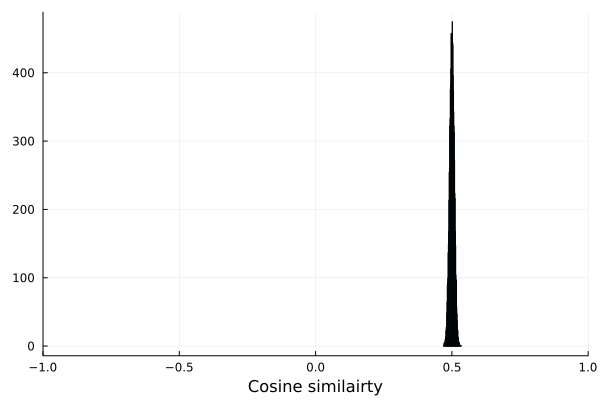
\includegraphics[scale = 0.7]{showcase}
    \caption{10000 cases of random 10000-dimensional bipolar vectors are made and each time implemented following example~\ref{eqn:ex1}. The resulting cosine similarities between $A$ and $A'$ are then plotted in a histogram.}
    \label{fig:exm1}
\end{figure}

We see that we can retrieve a lot of information with most of the cosine similarities centering around 0.5. Notice that two completely random HDVs would have a cosine similarity close to 0 just by stochastics. This result is not comparable to state-of-the-art accuracies but very efficient nonetheless as all of these calculations were done in less than 2 seconds. This same experiment was done with random binary 10000-dimensional vectors and it finished even faster as expected but retained the accuracy (similar \textit{Hamming distance} peak around 0.25).